\chapter{RESULTADOS E DISCUSS\~AO}
\label{cap:capitulo4}

\section{Desempenho dos modelos}
%Apresentar e comparar os resultados dos diferentes modelos utilizados.

Os resultados obtidos pelos modelos variaram significativamente em termos de precisão, tanto nas previsões pontuais quanto nos intervalos de previsão, refletindo diferentes graus de precisão para cada cenário analisado. Observou-se que a capacidade dos modelos em captar a variabilidade dos dados e as incertezas associadas às previsões foi particularmente sensível ao horizonte temporal considerado. Em horizontes mais curtos, como o de 1 dia, os modelos tenderam a apresentar um desempenho satisfatório, com baixos valores de erro e intervalos de previsão bem ajustados aos dados observados. No entanto, à medida que o horizonte de previsão foi expandido para 7 e 15 dias, notou-se um aumento substancial no erro percentual e uma maior discrepância entre os valores previstos e os observados, indicando dificuldades do modelo em captar tendências de longo prazo com a mesma precisão. Além disso, os intervalos de previsão tornaram-se menos eficientes na captura dos valores reais, especialmente nos horizontes mais extensos. Essa dinâmica de variação dos resultados será discutida em maior detalhe, dividida por bacia hidrográfica, o que permitirá uma análise mais específica das particularidades de cada região e a identificação de padrões específicos que possam influenciar o desempenho dos modelos.

\subsection{Rio Jequitinhonha}

Começando pela menor bacia estudada, os resultados mostraram-se bastante satisfatórios, especialmente no que tange à Regressão Linear, que se destacou com boas previsões tanto em termos pontuais quanto nos intervalos de previsão. Este modelo demonstrou uma boa capacidade de capturar a dinâmica hidrológica do rio, refletindo precisão nas métricas e um desempenho consistente para o horizonte de curto prazo. E com um tempo de execução baixo. O modelo simples \textit{Seasonal Naive} apresentou resultados aquém do esperado em todas as situações avaliadas, considerando a previsão pontual, porém, quando se considera os intervalos de previsão ele teve um bom desempenho, capturando o valor observado.

Saltando de 1 dia para 3 dias e depois para 7 dias, o modelo foi melhorando o resultado, tornando a piorar quando da previsão de 15 dias. É provável que o preenchimento de dados realizado aplicando a sazonalidade de anos anteriores tenha influenciado neste desempenho.

\begin{figure}[!h]
	\centering
	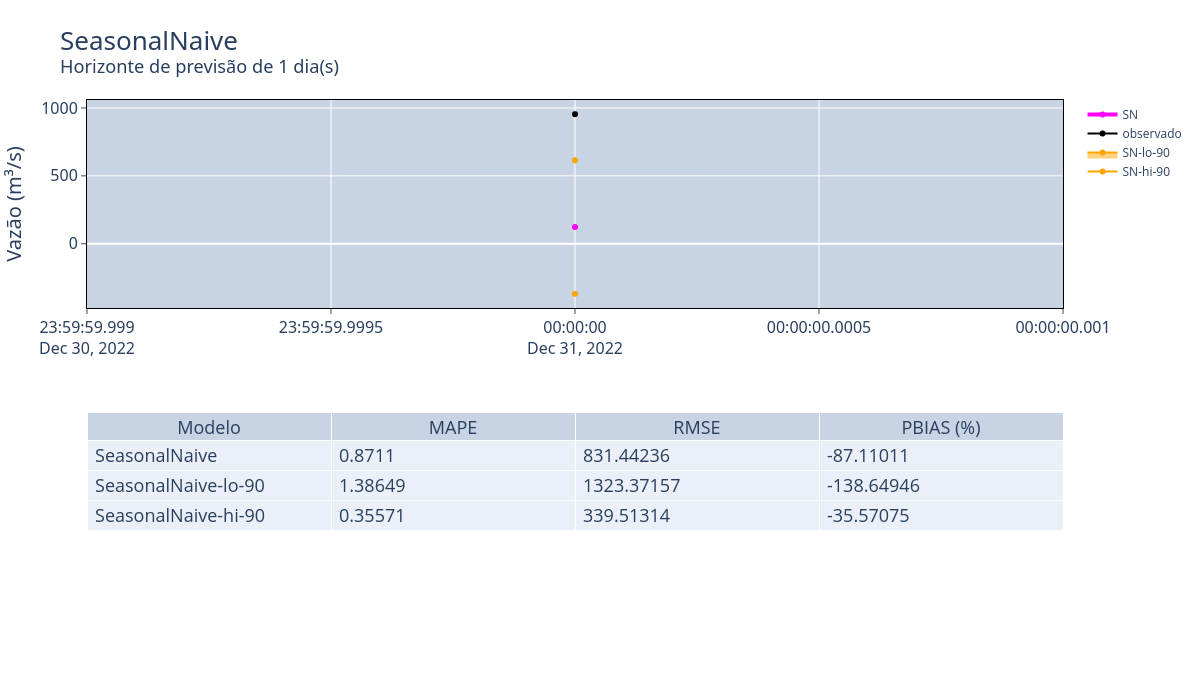
\includegraphics[scale=0.33]{Figuras/jequiti/resultados/SeasonalNaive_fh1.png}
	\caption{\textit{Seasonal Naive} para o horizonte de previsão de 1 dia\\(fonte: o autor)}
	\label{fig:jequiti_SeasonalNaive_fh1}
\end{figure}

\begin{figure}[!h]
	\centering
	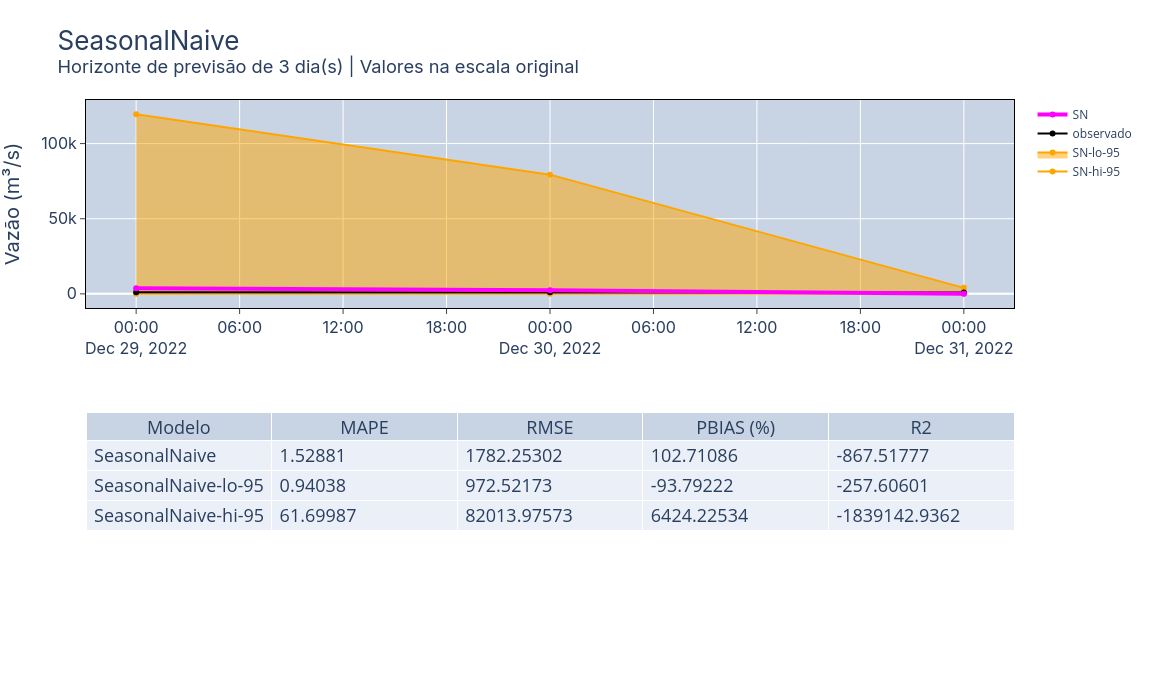
\includegraphics[scale=0.33]{Figuras/jequiti/resultados/SeasonalNaive_fh3.png}
	\caption{\textit{Seasonal Naive} para o horizonte de previsão de 3 dias\\(fonte: o autor)}
	\label{fig:jequiti_SeasonalNaive_fh3}
\end{figure}

\begin{figure}[!h]
	\centering
	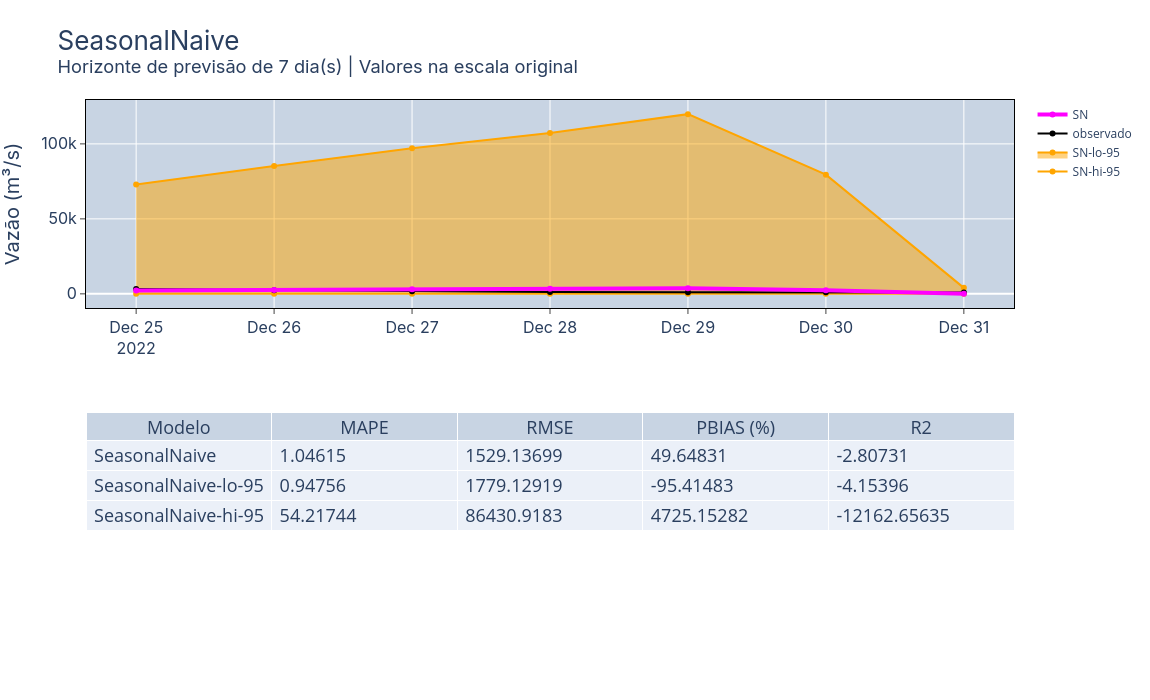
\includegraphics[scale=0.33]{Figuras/jequiti/resultados/SeasonalNaive_fh7.png}
	\caption{\textit{Seasonal Naive} para o horizonte de previsão de 7 dias\\(fonte: o autor)}
	\label{fig:jequiti_SeasonalNaive_fh7}
\end{figure}

\begin{figure}[!h]
	\centering
	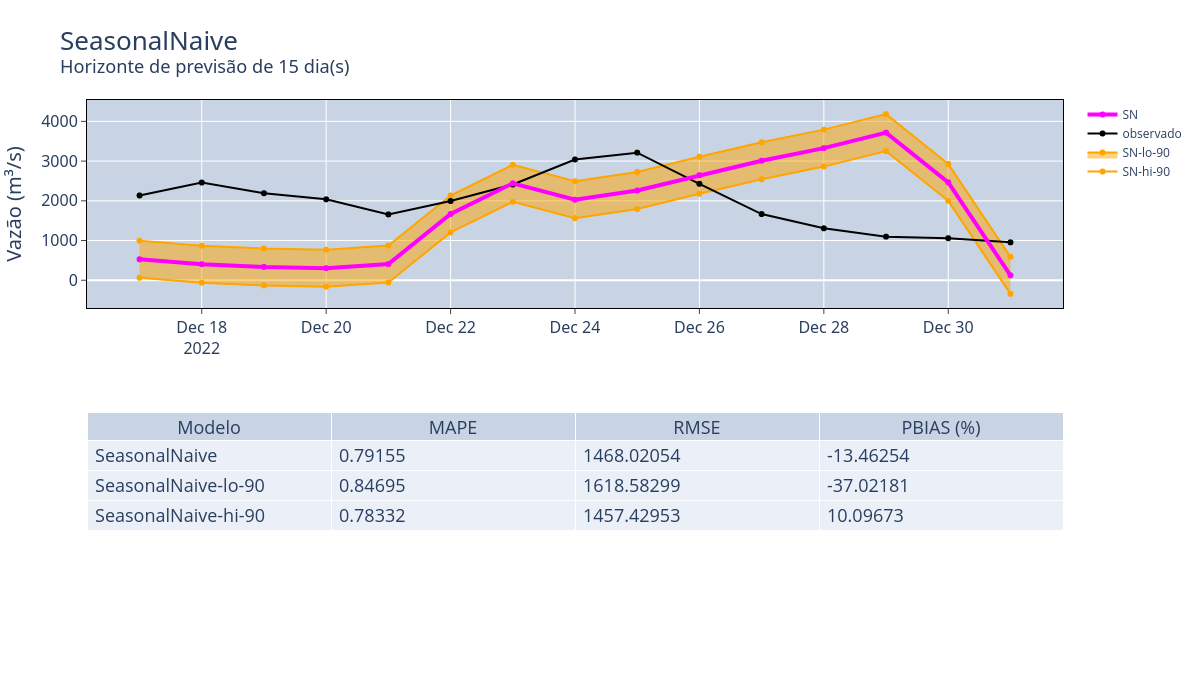
\includegraphics[scale=0.33]{Figuras/jequiti/resultados/SeasonalNaive_fh15.png}
	\caption{\textit{Seasonal Naive} para o horizonte de previsão de 15 dias\\(fonte: o autor)}
	\label{fig:jequiti_SeasonalNaive_fh15}
\end{figure}

%\begin{table}[!h]
%	\centering \small
%	\caption{Resultados SeasonalNaive - rio Jequitinhonha \\(fonte: o autor)}
%	\begin{tabular}{|l|r|r|r|r|r|r|} \hline 
%		\textbf{Horizonte} & \textbf{MAPE} & \textbf{RMSE} & \textbf{PBIAS} \\\hline
%		1 dia              & 0,871         & 831,44        & -87,11 \\\hline
%		3 dias             & 1,528         & 1872,25       & 102,71 \\\hline
%		7 dias             & 1,046         & 1529,13       & 49,64  \\\hline
%		15 dias            & 0,791         & 1468,02       & -13,46 \\\hline
%	\end{tabular}
%	\label{tab:sn_jequitinhonha_resultados}
%\end{table}

Os resultados obtidos utilizando o modelo de Regressão Linear mostraram-se promissores. Para o horizonte de previsão de 1 dia, o modelo apresentou uma superestimação nos valores previstos, conforme indicado pelo PBias positivo, e obteve um MAPE de apenas 4,7\%.(figura \ref{fig:jequiti_LinearRegression_fh1}) Este resultado demonstra uma precisão bastante elevada, com um erro percentual baixo, o que é muito satisfatório. À medida que o horizonte de previsão foi ampliado, observou-se um aumento no erro. No horizonte de 3 dias, o modelo manteve a tendência de superestimação e registrou um MAPE de 15,9\%, ainda dentro de um intervalo de erro que pode ser considerado aceitável, mas superior ao do horizonte de 1 dia.(figura \ref{fig:jequiti_LinearRegression_fh3}) Para o horizonte de 7 dias, o modelo continuou a superestimar os valores e obteve um MAPE de 26,5\%, indicando um erro mais pronunciado à medida que o período de previsão aumentou.(figura \ref{fig:jequiti_LinearRegression_fh7}) No horizonte de 15 dias, pela primeira vez, o modelo subestimou as previsões, refletido por um PBias negativo, e apresentou um MAPE de 60,3\%, o que representa um erro bastamte elevado.(figura \ref{fig:jequiti_LinearRegression_fh15}) Além disso, foi observado que, para os horizontes de 1, 3 e 7 dias, os intervalos de previsão capturaram os valores observados, enquanto que, para o horizonte de 15 dias, poucas vezes o valor observado esteve dentro da faixa de previsão calculada. Isso sugere que o modelo enfrentou dificuldades em captar as incertezas a partir dos dados de treinamento para previsões de longo prazo, mesmo ao considerar os intervalos de previsão, o que reflete uma limitação na capacidade de generalização do modelo para horizontes mais extensos.

\begin{figure}[!h]
	\centering
	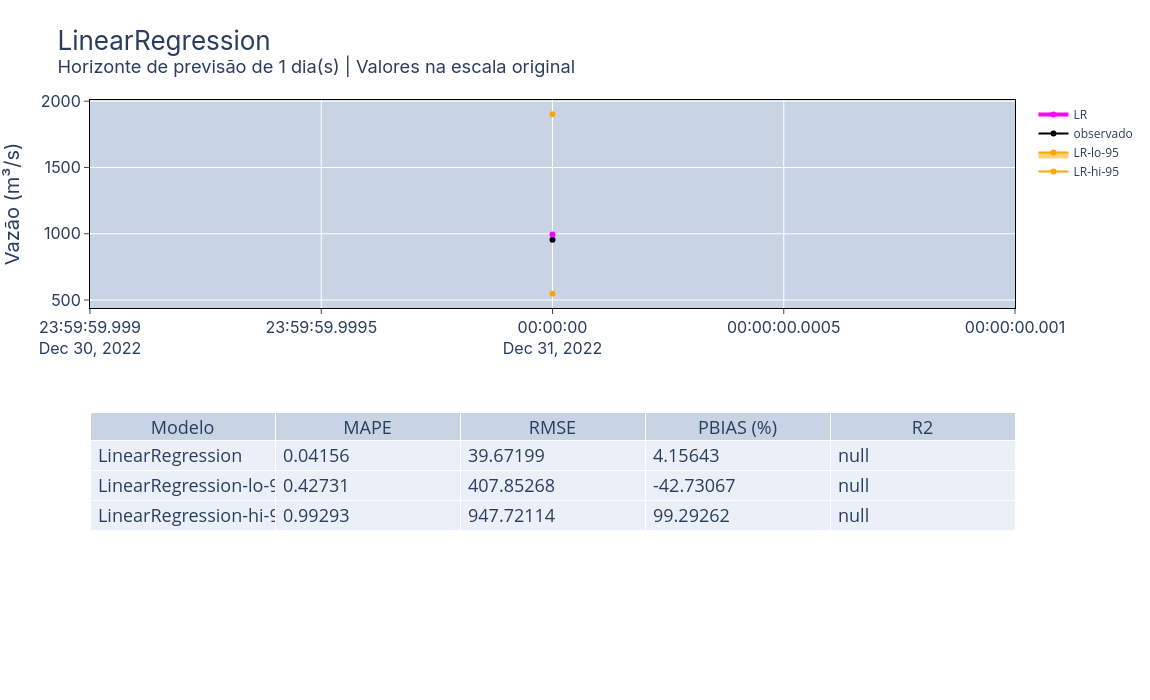
\includegraphics[scale=0.33]{Figuras/jequiti/resultados/LinearRegression_fh1.png}
	\caption{Regressão Linear para o horizonte de previsão de 1 dia\\(fonte: o autor)}
	\label{fig:jequiti_LinearRegression_fh1}
\end{figure}

\begin{figure}[!h]
	\centering
	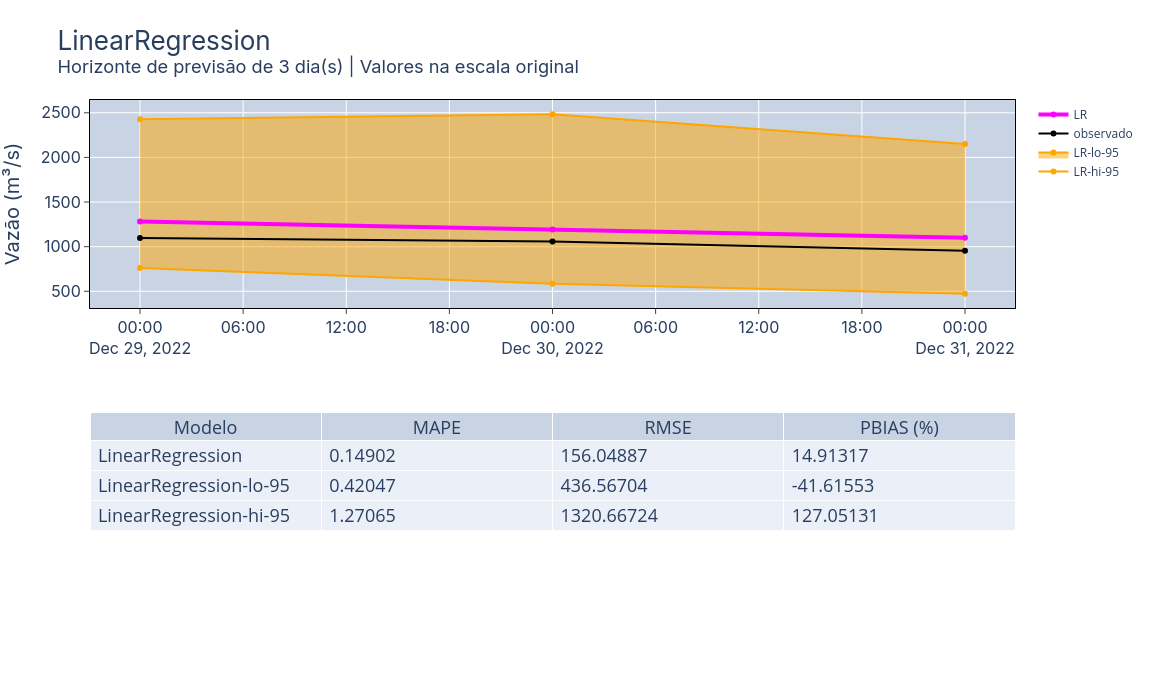
\includegraphics[scale=0.33]{Figuras/jequiti/resultados/LinearRegression_fh3.png}
	\caption{Regressão Linear para o horizonte de previsão de 3 dias\\(fonte: o autor)}
	\label{fig:jequiti_LinearRegression_fh3}
\end{figure}

\begin{figure}[!h]
	\centering
	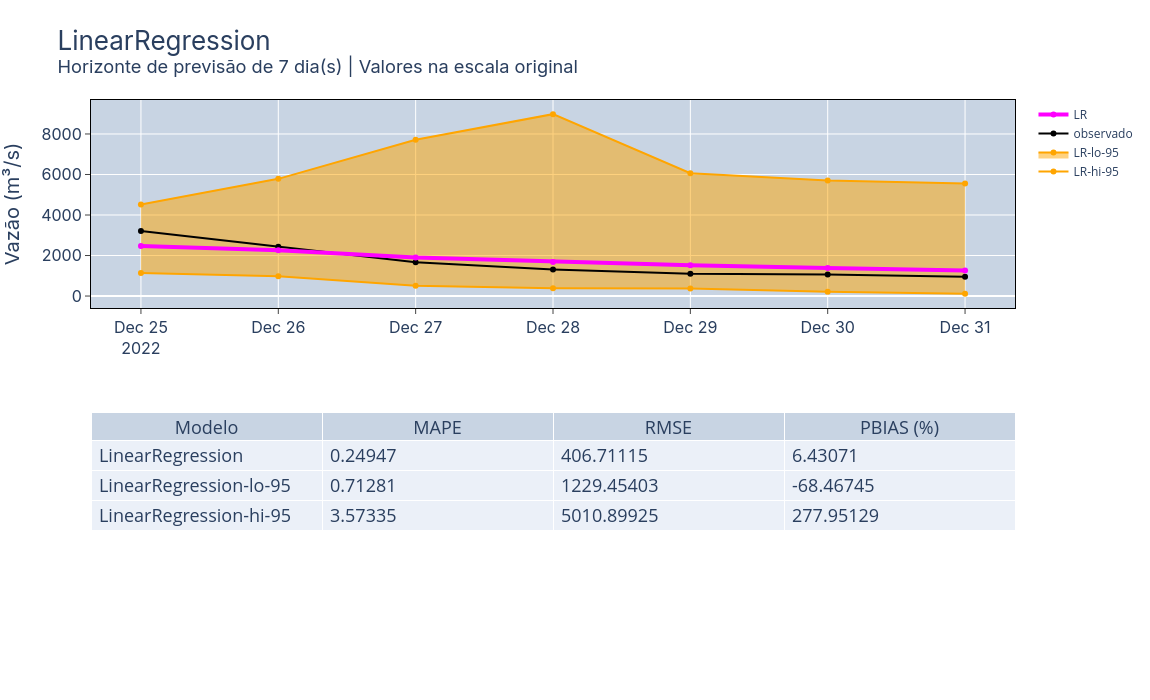
\includegraphics[scale=0.33]{Figuras/jequiti/resultados/LinearRegression_fh7.png}
	\caption{Regressão Linear para o horizonte de previsão de 7 dias\\(fonte: o autor)}
	\label{fig:jequiti_LinearRegression_fh7}
\end{figure}

\begin{figure}[!h]
	\centering
	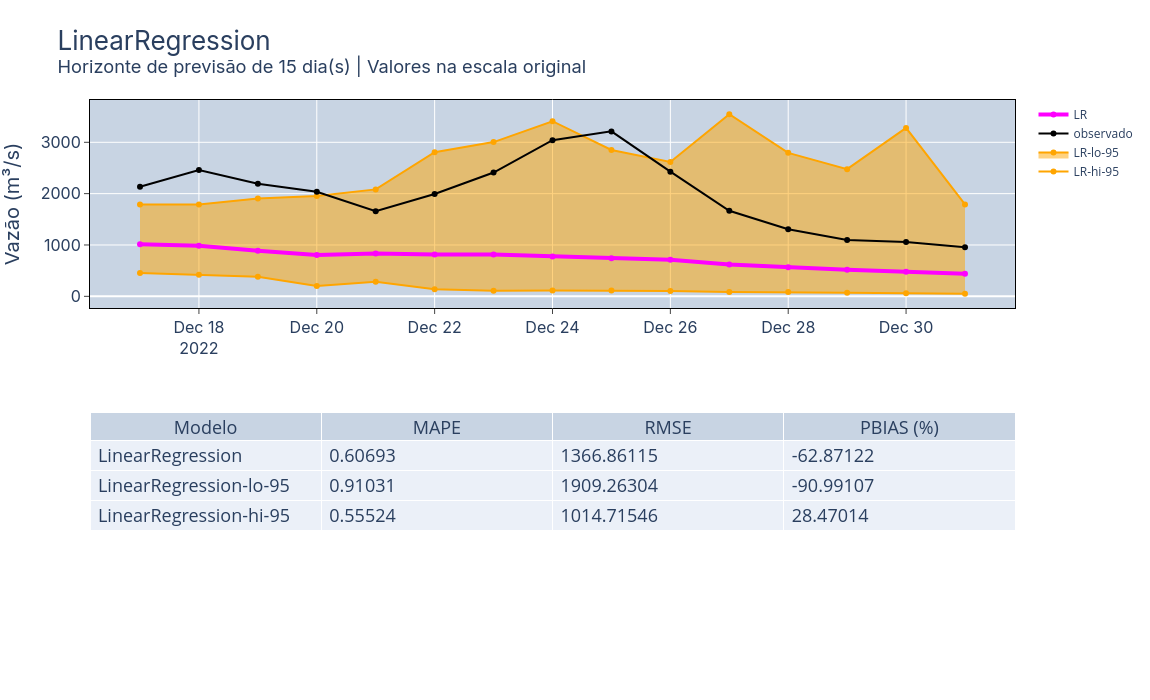
\includegraphics[scale=0.33]{Figuras/jequiti/resultados/LinearRegression_fh15.png}
	\caption{Regressão Linear para o horizonte de previsão de 15 dias\\(fonte: o autor)}
	\label{fig:jequiti_LinearRegression_fh15}
\end{figure}

Continuando a análise, agora os modelos principais do trabalho, ajustados com variáveis categóricas para melhor realizar as previsões a partir da sazonalidade.

Houve uma intercalação no desempenho dos resultados. Para o horizonte de 1 dia, o LightGBM apresentou um resultado melhor em relação ao CatBoost em todas as métricas. O intervalo de previsão também foi melhor pois capturou o valor observado, coisa que o CatBoost não fez.(figuras \ref{fig:jequiti_LGBMRegressor_fh1} e \ref{fig:jequiti_CatBoostRegressor_fh1})

Quando aumentou o horizonte para 3 dias, o CatBoost apresentou melhor desempenho, inclusive nos intervalos de previsão.(figura \ref{fig:jequiti_CatBoostRegressor_fh3})

\begin{figure}[!h]
	\centering
	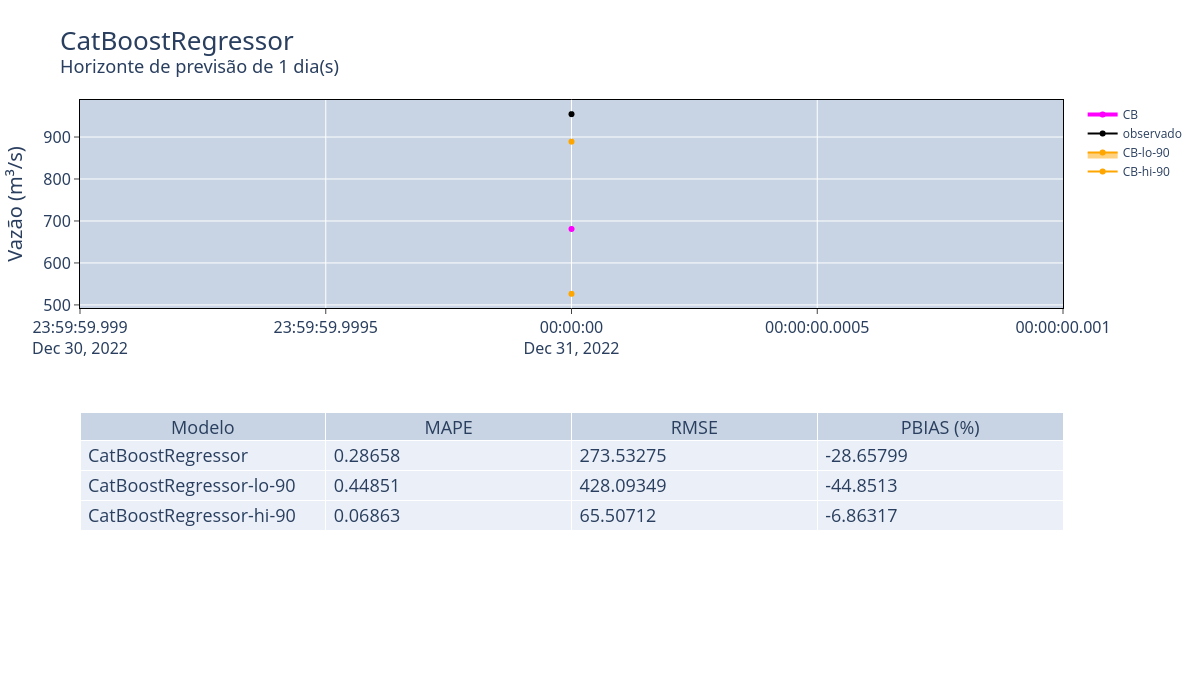
\includegraphics[scale=0.33]{Figuras/jequiti/resultados/CatBoostRegressor_fh1.png}
	\caption{CatBoost para o horizonte de previsão de 1 dia\\(fonte: o autor)}
	\label{fig:jequiti_CatBoostRegressor_fh1}
\end{figure}

\begin{figure}[!h]
	\centering
	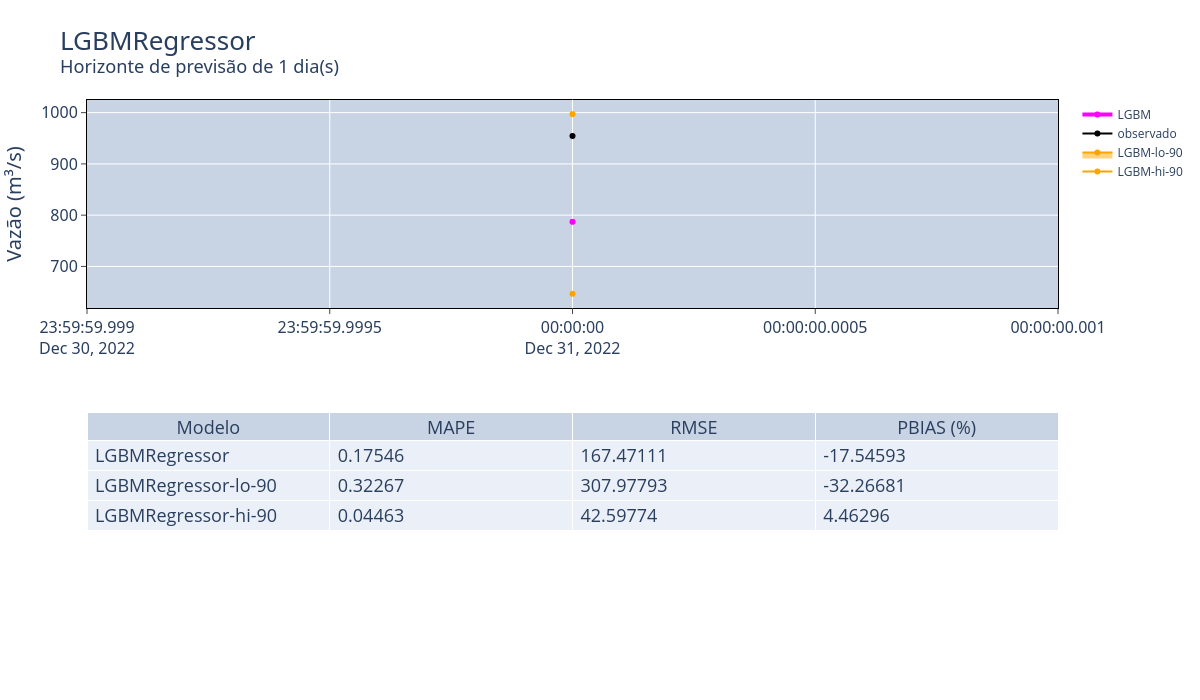
\includegraphics[scale=0.33]{Figuras/jequiti/resultados/LGBMRegressor_fh1.png}
	\caption{LightGBM para o horizonte de previsão de 1 dia\\(fonte: o autor)}
	\label{fig:jequiti_LGBMRegressor_fh1}
\end{figure}

\begin{figure}[!h]
	\centering
	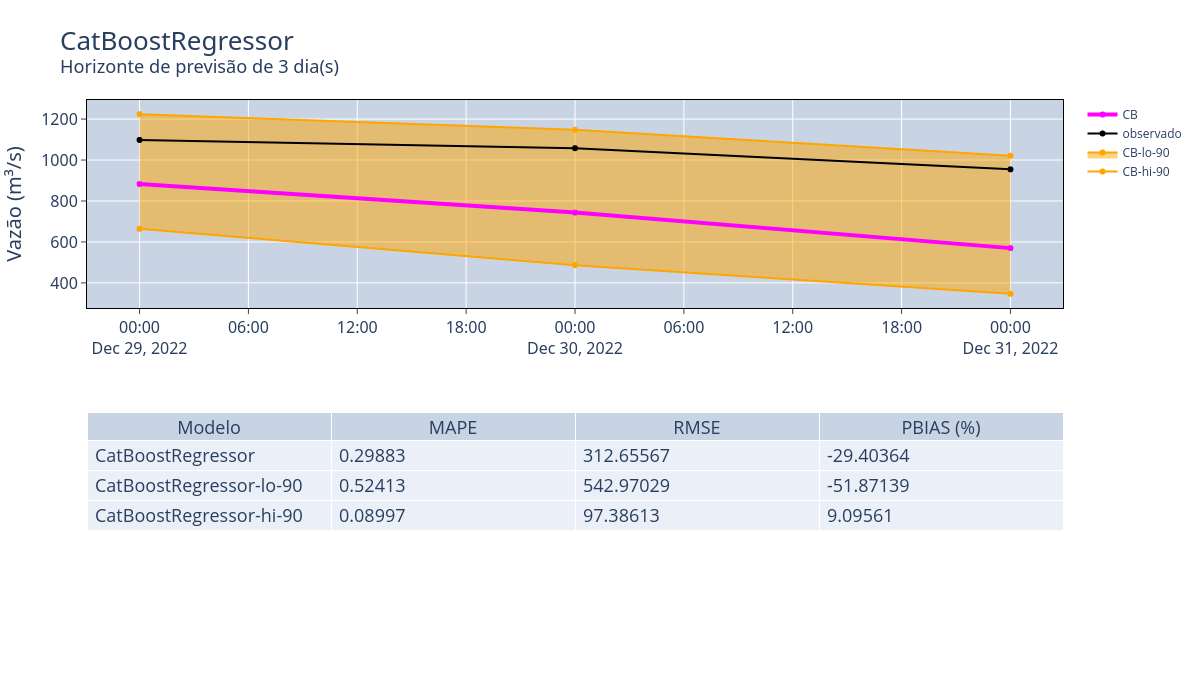
\includegraphics[scale=0.33]{Figuras/jequiti/resultados/CatBoostRegressor_fh3.png}
	\caption{CatBoost para o horizonte de previsão de 3 dias\\(fonte: o autor)}
	\label{fig:jequiti_CatBoostRegressor_fh3}
\end{figure}

\begin{figure}[!h]
	\centering
	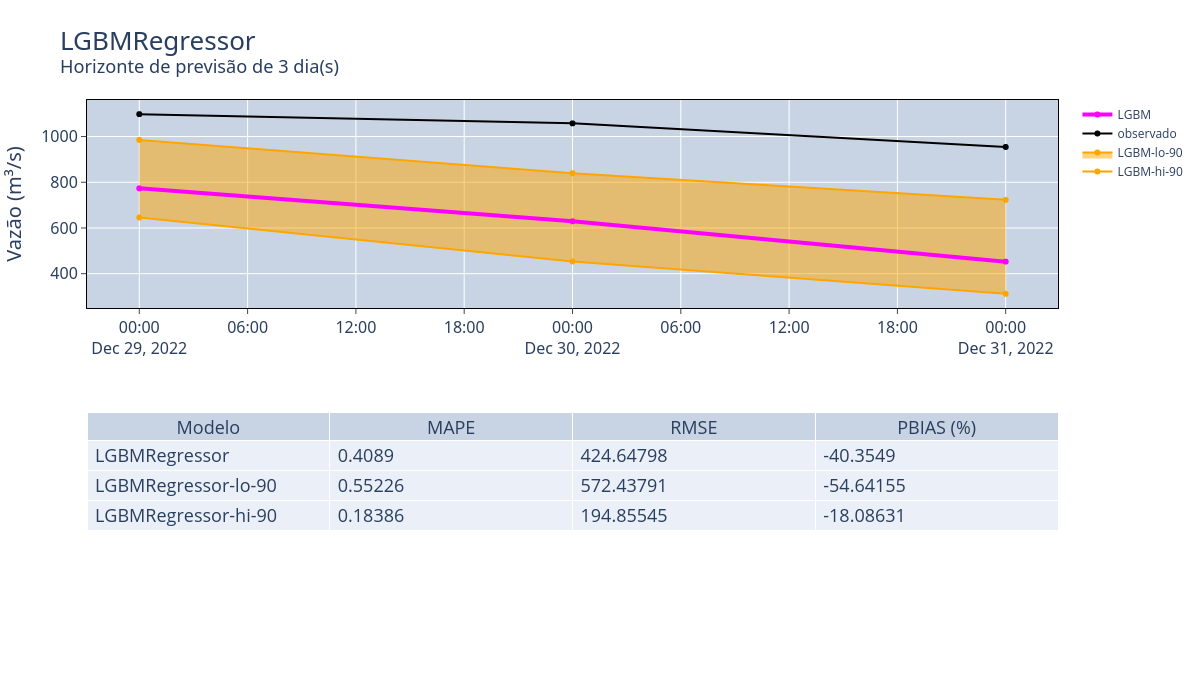
\includegraphics[scale=0.33]{Figuras/jequiti/resultados/LGBMRegressor_fh3.png}
	\caption{LightGBM para o horizonte de previsão de 3 dias\\(fonte: o autor)}
	\label{fig:jequiti_LGBMRegressor_fh3}
\end{figure}

\begin{figure}[!h]
	\centering
	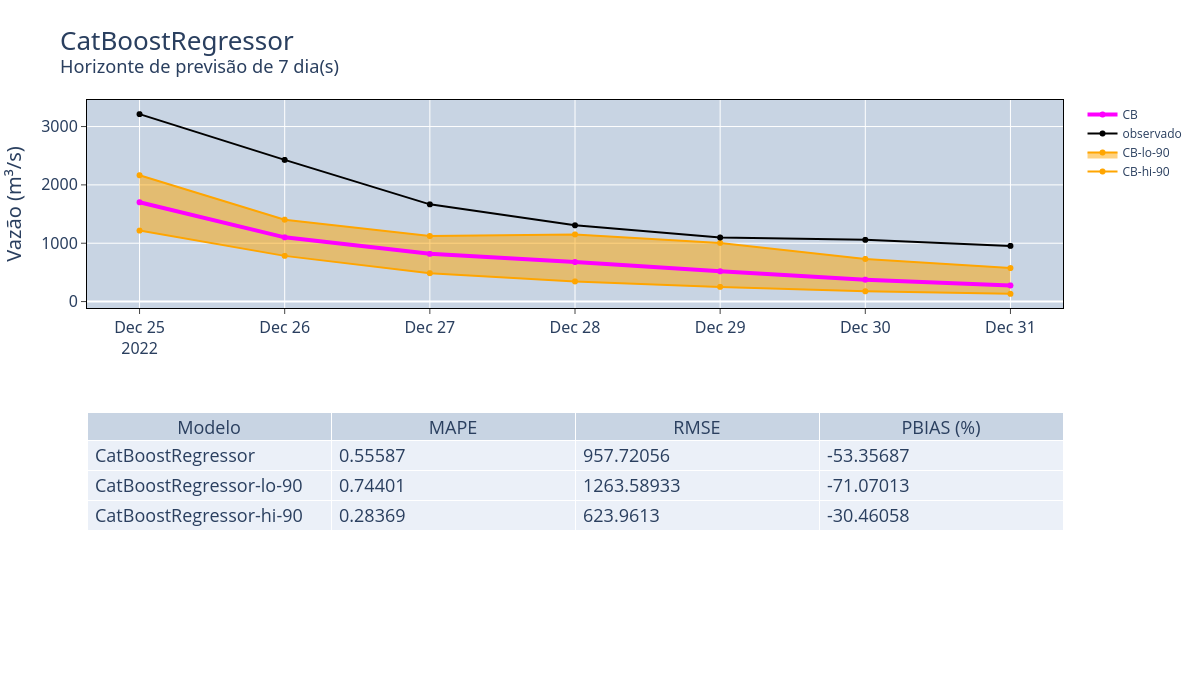
\includegraphics[scale=0.33]{Figuras/jequiti/resultados/CatBoostRegressor_fh7.png}
	\caption{CatBoost para o horizonte de previsão de 7 dias\\(fonte: o autor)}
	\label{fig:jequiti_CatBoostRegressor_fh7}
\end{figure}

\begin{figure}[!h]
	\centering
	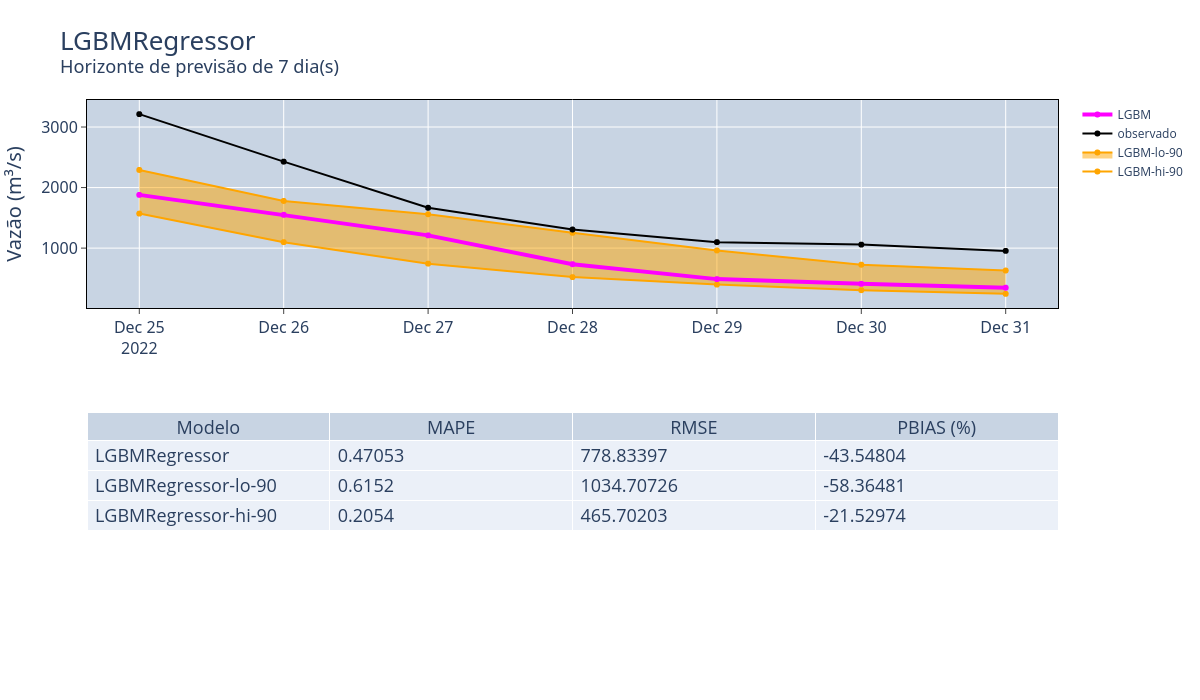
\includegraphics[scale=0.33]{Figuras/jequiti/resultados/LGBMRegressor_fh7.png}
	\caption{LightGBM para o horizonte de previsão de 7 dias\\(fonte: o autor)}
	\label{fig:jequiti_LGBMRegressor_fh7}
\end{figure}

\begin{figure}[!h]
	\centering
	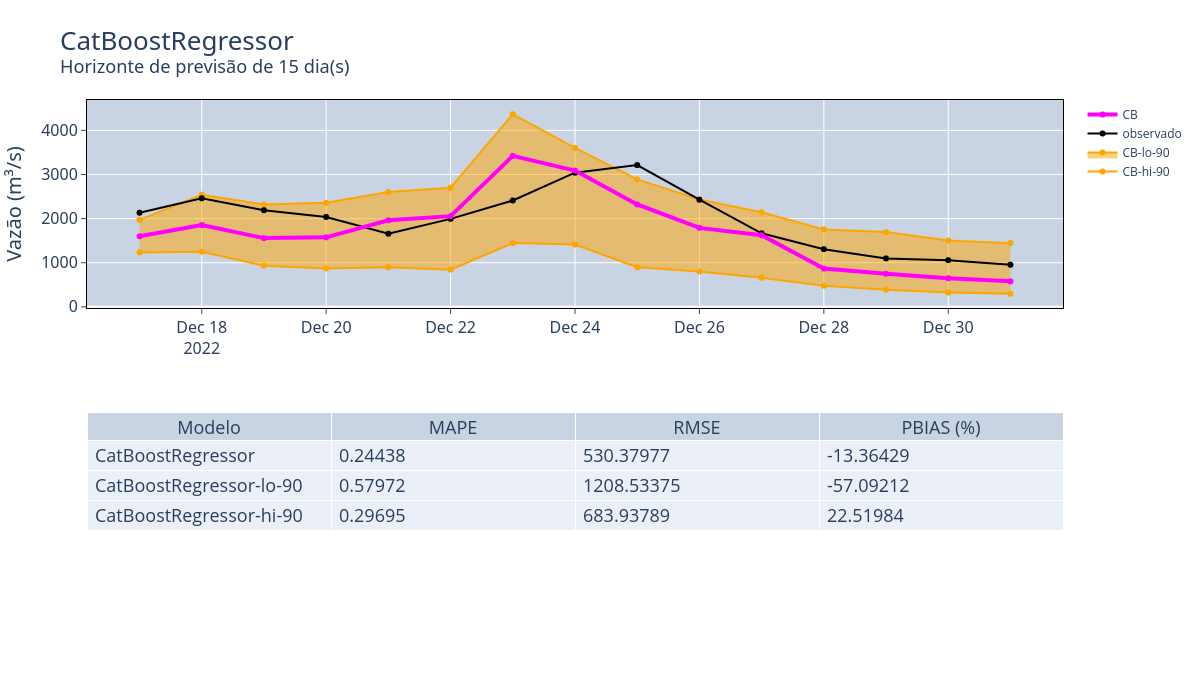
\includegraphics[scale=0.33]{Figuras/jequiti/resultados/CatBoostRegressor_fh15.png}
	\caption{CatBoost para o horizonte de previsão de 15 dias\\(fonte: o autor)}
	\label{fig:jequiti_CatBoostRegressor_fh15}
\end{figure}

\begin{figure}[!h]
	\centering
	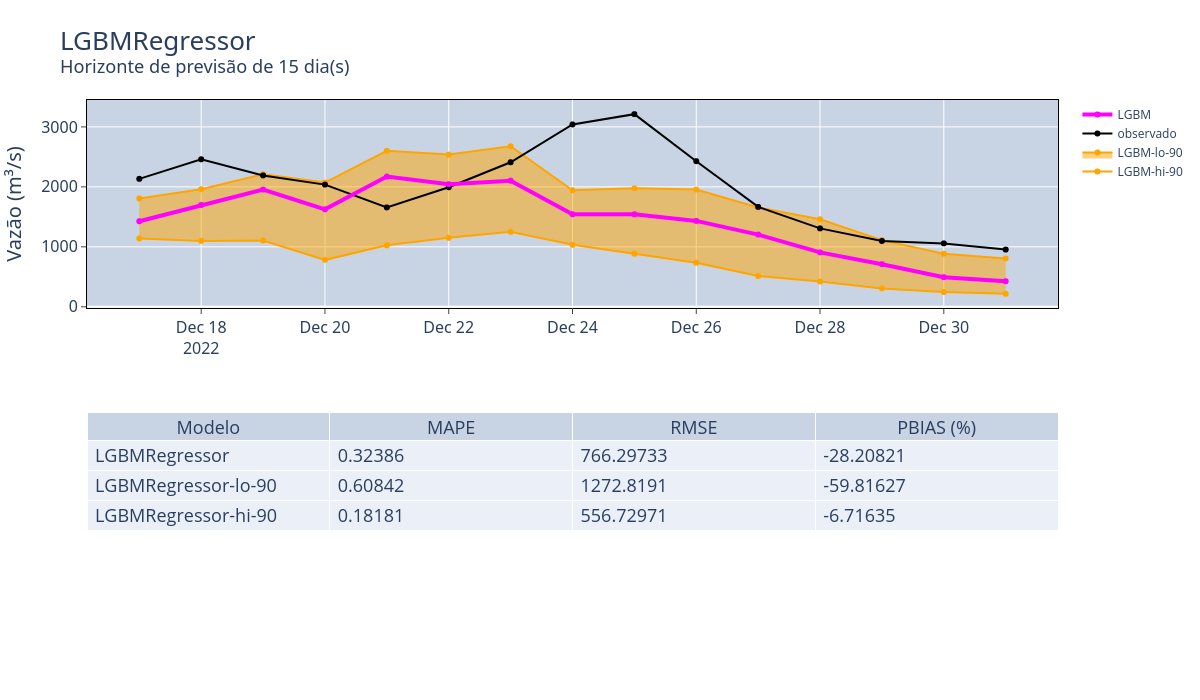
\includegraphics[scale=0.33]{Figuras/jequiti/resultados/LGBMRegressor_fh15.png}
	\caption{LightGBM para o horizonte de previsão de 15 dias\\(fonte: o autor)}
	\label{fig:jequiti_LGBMRegressor_fh15}
\end{figure}
\clearpage

Os intervalos de previsão estreitos denotam que a previsão não captou todas as incertezas presentes na dinâmica do fenômeno.\cite{RobHyndman_prediction_intervals}

\section{Importância das variáveis}
%Analisar a importância das variáveis contínuas e categóricas na previsão (feature importance).

\section{Discuss\~ao dos resultados}
%Interpretar os resultados e discutir as limitações. Se possível, comparar com estudos anteriores.